%%%%%%%%%%%%%%%%%%%%%%%%%%%%%%%%%%%%%%%%%%%%
% LaTeX Generator 

% Créé par Arnaud Ibakuyumcu
% ENSIMAG 2A IF
%%%%%%%%%%%%%%%%%%%%%%%%%%%%%%%%%%%%%%%%%%%%

 \documentclass[a4paper,12pt]{article}

 %---Package Generique ---% 

 \usepackage[francais]{babel}
 \usepackage[utf8]{inputenc}
 \usepackage[babel=true]{csquotes}
 \usepackage{amsmath}
 \usepackage{amssymb}
 \usepackage{hyperref}
 \usepackage{float}
 \usepackage{graphicx}
 \usepackage{enumitem} %% Pour changer les puces des enum
 \graphicspath{{images/}}

 \usepackage{fancybox} %% Pour les encadrés : Usage \shadowbox{}
 \usepackage{fancyhdr} %% Pour les en-tetes et pieds
 \usepackage{array,multirow,makecell} %% Pour les tableaux à lignes fusionnées
 \setcellgapes{1pt}
 \makegapedcells

 %--- Partie Page de Code ---%
\usepackage{listings}
\usepackage{color}

\definecolor{dkgreen}{rgb}{0,0.6,0}
\definecolor{gray}{rgb}{0.5,0.5,0.5}
\definecolor{mauve}{rgb}{0.58,0,0.82}
%--- Definir les reglages ---%
\lstset{frame=tb,
language=C++,
aboveskip=3mm,
belowskip=3mm,
showstringspaces=false,
columns=flexible,
basicstyle={\small\ttfamily},
numbers=none,
numberstyle=\tiny\color{gray},
keywordstyle=\color{blue},
commentstyle=\color{dkgreen},
stringstyle=\color{mauve},
breaklines=true,
breakatwhitespace=true,
tabsize=3
}

 %--- Structure de la page ---%

 \topmargin -1.5 cm
 \textwidth 18 cm
 \textheight 25 cm
 \oddsidemargin -1 cm
 \marginparwidth -1 cm
 \evensidemargin -1 cm
 \parindent 0 cm

 \pagestyle{fancy}
 \renewcommand{\headrulewidth}{1pt}
 \fancyhead[C]{}
 \fancyhead[R]{Team 9}
 \fancyhead[L]{PEPS : Multimonde21}

 \renewcommand{\footrulewidth}{1pt}
 \fancyfoot[C]{ENSIMAG}
 \fancyfoot[L]{}
 \fancyfoot[R]{\textbf{Page : \thepage}}

 %---Raccourci Commande---%

 \newcommand{\R}{\mathbb{R}}
 \newcommand{\N}{\mathbb{N}}
 \newcommand{\A}{\mathbf{A}}
 \newcommand{\B}{\mathbf{B}}
 \newcommand{\C}{\mathbf{C}}
 \newcommand{\D}{\mathbf{D}}
 \newcommand{\ub}{\mathbf{u}}
 \newcommand{\vs}{{\bf : } \vspace*{3mm} \\}
 \newcommand{\HRule}{\rule{\linewidth}{0.5mm}} %% Pour la page de garde

 %--- Debut du document ---% 

 \begin{document}

\begin{titlepage}
\begin{center}


\includegraphics[width=0.35\textwidth]{logo}~\\[2.5cm] %% Modifier les réglages

\textsc{\LARGE ENSIMAG}\\[1.5cm]
\textsc{\Large }\\[0.5cm]

%Title
\HRule \\[0.4cm]

{\Huge \bfseries \textsf{PEPS : Multimonde21}\\[0.5cm]
\texttt{ Présentation\\
Version Beta} \\[0.4cm] }

\HRule \\[1.5cm]

\begin{minipage}{0.4\textwidth}
\begin{center} \large
\emph{IF - Groupe 9}\\[2cm]
Ibakuyumcu Arnaud \\
Lhuillery Paul \\
Ruimy Benjamin \\
Voong Kwan \\
Rattanatray Ayutaya
\end{center}
\end{minipage}
\begin{minipage}{0.4\textwidth}
\end{minipage}

\vfill

\large {25/01/2017 }

\end{center}

\end{titlepage}
 \newpage

 %---Sommaire---%

 \tableofcontents %Compiler deux fois pour avoir la table des matières
 \newpage

 %--- Commencer a ecrire ici ---% 
 \part{Présentation du projet}
 \section{Le produit Multimonde}
 \newpage
\part{Mathématiques}
\section{Modélisation du produit multi-économies}
Le produit {\tt multimonde21} met en jeu des sous-jacents répartis sur plusieurs économies (et devises). Contrairement à la couverture en delta classique sur une seule économie, le portefeuille de réplication induit un achat de titres étrangers et par cette occasion une exposition au risque de change. \\
La modélisation doit donc faire intervenir de nouveaux actifs risqués : les changes.
\subsection{Notations}
On pose $H$ le pay off du produit multimonde.
On posera pour la suite les indices $(S_k(t))_{k=1,\ldots,6}$ du panier du produit et leur économie respective dans l'ordre suivant : 
\begin{enumerate}
\item Eurostock50 (EUR)
\item Ftse (GBP)
\item P500 (USD)
\item Hangseng (CNY)
\item Nikkei (JPY)
\item SPASX200 (AUD)
\end{enumerate}
On notera aussi $(r_k(t))_{k=1,\ldots,6}$ les taux sans risque de chaque économie et $(X_k(t))_{k=1,\ldots,6}$ les changes associés pour revenir à la monnaie domestique : l'euro.\footnote{Bien évidemment $X_1(t)=1$ et ne sera pas utilisé puisque $S_1$ est un actif domestique} \\[2mm]
Le pay off faisant intervenir seulement les performances de ces indices on peut noter $H=u(S_1,\ldots,S_6)$.
\subsection{Modèle de Black\&Scholes}
On utilisera la modélisation classique de Black\& Scholes pour écrire la dynamique de prix des différents actifs. 
\subsubsection{Sous probabilité historique}
On modélise le marché sous l'espace de probabilité historique filtré $(\Omega,(\mathcal{F}_t)_t,\mathbb{P})$ de la façon suivante : 
\begin{itemize}[label=$\star$]
\item Actif risqué domestique : \begin{center} $dS_1(t)=S_1(t)\left(\mu^1(t)dt+\widehat{\sigma}^1(t).dW(t)\right)$ \end{center}
\item Taux de change : \begin{center} $\left(\forall k \in \{2,\ldots,6\}\right)dX_k(t)=X_k(t)\left(\mu^{X_k}(t)dt+\widehat{\sigma}^{X_k}(t).dW(t)\right)$\end{center}
\item Actifs risqués étrangers : \begin{center} $\left(\forall k \in \{2,\ldots,6\}\right)dS_k(t)=S_k(t)\left(\mu^k(t)dt+\widehat{\sigma}^k(t).dW(t)\right)$\end{center}
\newpage
\item Actifs non risqués : \begin{center} $\left(\forall k \in \{1,\ldots,6\}\right) dR_k(t)=R_k(t)r^k(t)dt$\end{center}
\end{itemize}
Où $\widehat{\sigma}^k$ la $k$-ieme ligne et $\widehat{\sigma}^{X_k}$ la $(k+5)$-ieme ligne de $\sigma$ et $W(t)$ est un MB à $11$ dimensions.\\[2mm]
Par la suite on supposera l'ensemble des tendances $\mu$ et la matrice de volatilité $\sigma$ déterministes et constants au cours du temps.

\subsubsection{Reconsidération des actifs en euros}
On se place pour la suite dans l'économie domestique, pour cela il faut que chacun des actifs considérés soit exprimé en euro : on use donc des taux de changes pour convertir les actifs risqués. \\
La dynamique sous probabilité historique devient alors la suivante après application de la formule d'Itô :  \footnote{L'ensemble des actifs sont dans l'économie domestique désormais} 
\begin{itemize}[label=$\star$]
\item  $dS_1(t)=S_1(t)\left(\mu^1dt+\widehat{\sigma}^1.dW(t)\right)$ \\
\item $dR_1(t) = R_1(t)r^1(t)dt$ \\
\item $\left(\forall k \in \{2,\ldots,6\}\right)d(X_kS_k)(t)=X_k(t)S_k(t)\left[\left(\mu^k + \mu^{X_k} + \widehat{\sigma}^k.\widehat{\sigma}^{X_k}\right)dt+\left(\widehat{\sigma}^k+\widehat{\sigma}^{X_k}\right).dW(t)\right]$ \\
\item  $\left(\forall k \in \{2,\ldots,6\}\right)d(X_kR_k)(t)=X_k(t)R_k(t)\left[\left(\mu^{X_k}+r^k(t)\right)dt+\widehat{\sigma}^{X_k}(t).dW(t)\right]$
\end{itemize} \vspace*{2mm} 
On pose alors le vecteur des trends et la matrice des volatilités dans l'univers euro : \begin{center} $\overset{\sim}{\mu}(t) = 
\begin{bmatrix}
\mu_1 \\
\left(\mu_2+\mu^{X_2}+\widehat{\sigma}^2.\widehat{\sigma}^{X_2}\right) \\
\vdots \\
\left(\mu_6+\mu^{X_6}+\widehat{\sigma}^6.\widehat{\sigma}^{X_6}\right) \\
\left(\mu^{X_2}+r^2(t)\right) \\
\vdots \\
\left(\mu^{X_6}+r^6(t)\right)
\end{bmatrix}$
 et $\overset{\sim}{\sigma} = 
\begin{bmatrix}
\left(\widehat{\sigma}^1\right)^T \\
\left(\widehat{\sigma}^2+\widehat{\sigma}^{X_2}\right)^T \\
\vdots \\
\left(\widehat{\sigma}^6+\widehat{\sigma}^{X_6}\right)^T \\
\left(\widehat{\sigma}^{X_2}\right)^T \\
\vdots \\
\left(\widehat{\sigma}^{X_6}\right)^T
\end{bmatrix}
$ 
\end{center}

\subsection{Prix sous probabilité risque neutre}
On suppose que la matrice de volatilité $\overset{\sim}{\sigma}$ est inversible et que $\overset{\sim}{\sigma}.\overset{\sim}{\sigma}^T$ est minoré au sens des matrices symétriques. \\
Sous ces hyposthèses, le marché est complet et il existe une probabilité risque neutre domestique $Q^d$ sous laquelle les actifs domestiques actualisés au taux sans risque domestique sont des martingales. \\
La prime de risque associé est $\lambda (t)=\overset{\sim}{\sigma}^{-1}.\left(r^1(t).\mathbf{1}_{11}-\overset{\sim}{\mu} (t)\right)$. 
\newpage
\subsubsection{Dynamique sous $Q^d$}
On note $W^d(t) = W(t)+\int\limits_0^t\lambda(t)dt$ le mouvement brownien associé au nouvel espace risque neutre.\\
Les dynamiques des actifs sous cette probabilités sont alors : 
\begin{itemize}[label=$\star$]
\item  $dS_1(t)=S_1(t)\left(r^1(t)dt+\widehat{\sigma}^1.dW^d(t)\right)$ \\
\item $dR_1(t) = R_1(t)r^1(t)dt$ \\
\item $\left(\forall k \in \{2,\ldots,6\}\right)d(X_kS_k)(t)=X_k(t)S_k(t)\left[r^1(t)dt+\left(\widehat{\sigma}^k+\widehat{\sigma}^{X_k}\right).dW^d(t)\right]$ \\
\item  $\left(\forall k \in \{2,\ldots,6\}\right)d(X_kR_k)(t)=X_k(t)R_k(t)\left[r^1(t)dt+\widehat{\sigma}^{X_k}.dW^d(t)\right]$
\end{itemize} \vspace*{2mm} 

\subsubsection{Portefeuille de couverture et prix}
Le portefeuille de couverture $V$ est alors constitué des actifs suivants en $t$ : 
\begin{itemize}[label=$\bullet$]
\item $\Delta_1(t)$ actifs $S_1$
\item $\Delta_k(t)$ actifs $X_kS_k$ pour $k\in\{2,\ldots,6\}$
\item $\Delta_{k+6}(t)$ actifs $X_kR_k$ pour $k\in\{1,\ldots,6\}$
\end{itemize}
En supposant ce portefeuille de couverture autofinancé et admissible on a alors que le prix du portefeuille actualisé au taux sans risque domestique $\overset{\sim}{V}$ est une martingale sous $Q^d$. \\[1mm]
Dès lors on a l'égalité suivante pour $t<T$ : $\overset{\sim}{V}(t) = E^{Q^d}\left[\overset{\sim}{V}(T)\mid\mathcal{F}_t\right]$. \\[2mm]
Si on impose $V(T)=H$ alors par absence d'oportunité d'arbitrage, le prix du produit est le prix du portefeuille de couverture $V(t)$ et on a l'égalité suivante : \begin{center}
$Prix(t) = V(t) = E^{Q^d}\left[\frac{R_1(t)}{R_1(T)}H\mid\mathcal{F}_t\right]$
\end{center}
\subsubsection{Calcul des deltas}
Pour intégrer les sous-jacents du portefeuille de couverture on peut utiliser une nouvelle fonction $g(s,x,y)$ tel que :
\begin{center}
$g\left(S_1,\left(X_2S_2\ldots,X_6S_6\right),\left(X_2R_2,\ldots,X_6R_6\right)\right) = u\left(S_1,\left(\frac{X_2S_2}{X_2R_2}*R_2\right),\ldots,\left(\frac{X_6S_6}{X_6R_6}*R_6\right)\right) = H$
\end{center}
Dans ce cas, le prix en $t$ vaut $prix(t)=\phi\left(S_1(t),\left((X_2S_2)(t)\ldots,(X_6S_6)(t)\right),\left((X_2R_2)(t),\ldots,(X_6R_6)(t)\right)\right)$ et on obtient les égalités suivantes : \\
\begin{itemize}[label=$\bullet$]
\item $\Delta_1(t)=\frac{\partial\phi}{\partial s}(t)$ \\
\item $\left(\forall k\in\{2,\ldots,6\}\right)\,\Delta_k(t)=\frac{\partial\phi}{\partial x_{k-1}}(t)$ \\
\item $\left(\forall k\in\{2,\ldots,6\}\right)\,\Delta_{k+6}(t)=\frac{\partial\phi}{\partial y_{k-1}}(t)$ \\
\item $\Delta_7(t)=\frac{1}{R_1(t)}\left(V(t)-\left(\Delta_1S_1(t)+\sum\limits_{k=2}^6\Delta_k(t)(X_kS_k)(t)+\Delta_{k+6}(t)(X_kR_k)(t)\right)\right)$
\end{itemize} \vspace*{3mm}
On montre qu'avec cette stratégie, le portefeuille est autofinancé, admissible et réplique le pay off $H$. C'est donc un portefeuille de couverture du produit {\tt multimonde21}.
\newpage
\subsection{Choix du modèle des taux sans risques}
Dans notre modèle, on utilisera en premier lieu des modèles de courbe de taux déterministes. \\
On rappelle que le prix $B(t,T)$ en $t$ d'un ZC d'échéance $T$ s'écrit : 
\begin{center}
$B(t,T) = e^{-\int_t^Tr_sds}$ ou $B(t,T) = e^{-R(t,T).(T-t)}$
\end{center}
Où $r_t$ est le taux instantané et $R(t,T)$ le taux moyen entre $t$ et $T$. \\

En univers déterministe, on a par absence d'opportunité d'arbitrage la relation suivante : 
\begin{center}
$\left(\forall t<T\right)\;B(0,T)=B(0,t)B(t,T)$
\end{center}
On en déduit en particulier la relation suivante : 
\begin{center}
$\left(\forall t<T\right)\;R(t,T)=\frac{R(0,T)T-R(0,t)t}{T-t}$
\end{center}
Ainsi, la plupart des modèles de courbes donnent une formule pour $R(0,t)$.
\subsubsection{Courbe des taux plate}
Dans ce modèle, on suppose la courbe des taux constante, c'est à dire que :
\begin{center}
$\left(\forall t<T\right)$ on a $r_t = r$ et $R(t,T)=r$
\end{center}

C'est le modèle le plus simple et le seul paramètre à estimer est $r$. \\
Dans la version Beta c'est ce modèle qui sera utilisé pour chacune des devises. \\[2mm]
\begin{center}
\begin{tabular}{c}
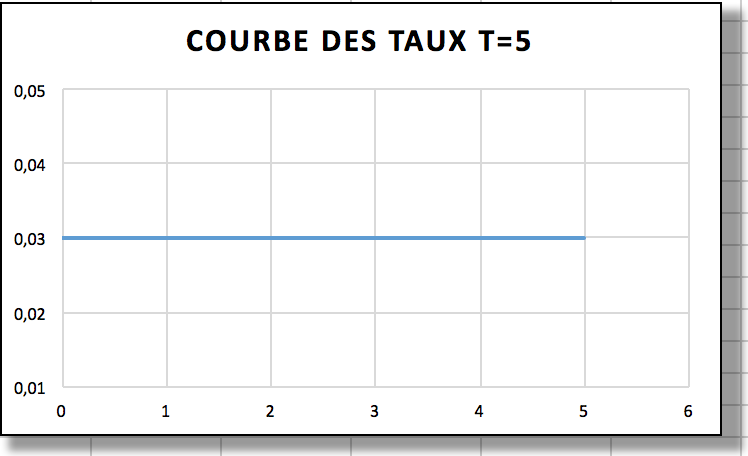
\includegraphics[scale=0.7]{constR} \\
Figure 1 : Courbe des taux plate avec $r=0.03$
\end{tabular}
\end{center}
\newpage
\subsubsection{Modèle GAMTAUX}
Le modèle de {\sf GAMTAUX} a été établie par Nicole El Karoui et le modèle de taux moyen s'écrit de la manière suivante : 
\begin{center}
$R(0,t)=r_{inf} - S.G_1(t) + \gamma.G_2(t)$ \\[2mm] 
avec $G_1(t)=\frac{\left(1-e^{-at}\right)}{at}$ et $G_2(t)=\frac{\left(1-e^{-at}\right)^2}{4at}$
\end{center}
Où $r_{inf}$ est le taux court, $S$ le spread avec le taux long, $\gamma$ un paramètre de courbure. \\

Le paramètre $a$ a été fixé à $0.4$ après de nombreux tests statistiques, les autres paramètres doivent être estimés. \\
Ci-dessous sont présentés les courbes $R(0,T)$ sous le modèle de {\sf GAMTAUX} en fonction des différents paramètres. \\[2mm]
\begin{center}
\begin{tabular}{cc}
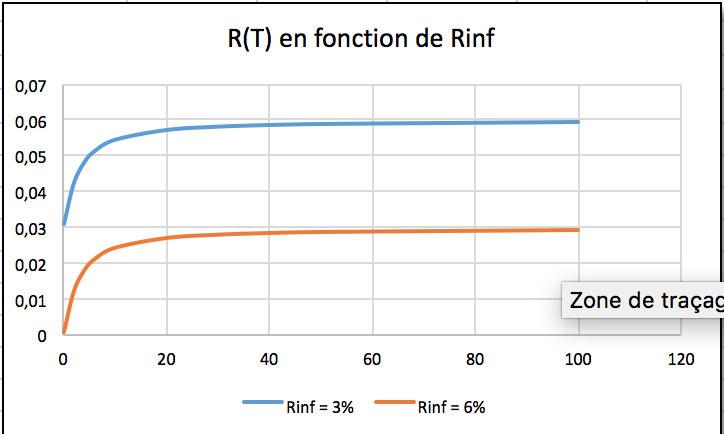
\includegraphics[scale=0.7]{Rrinf} & 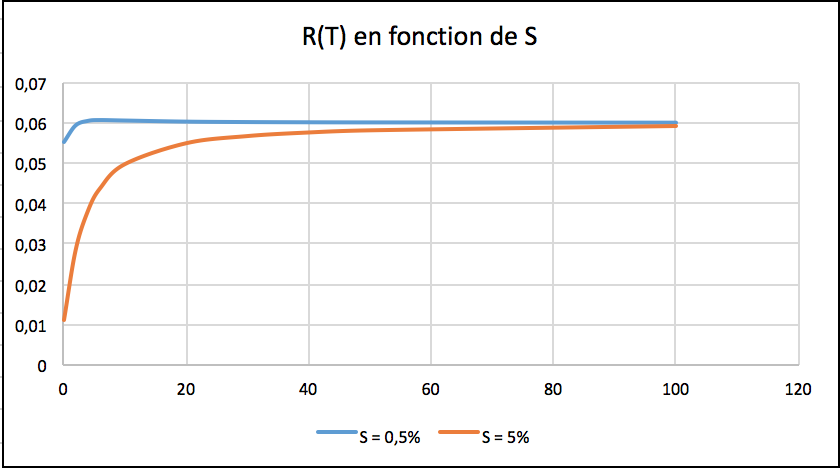
\includegraphics[scale=0.64]{Rs} \\
Figure 2 : Courbe en fonction de $r_inf$ & Figure 3 : Courbe en fonction de $S$ 
\end{tabular} \vspace*{5mm} \\
\begin{tabular}{c}
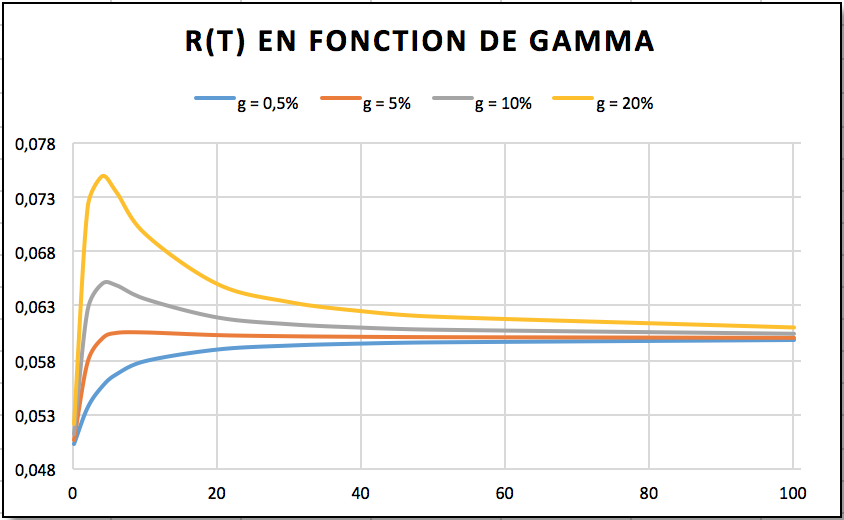
\includegraphics[scale=0.7]{Rgamma} \\
Figure 4 : Courbe en fonction de $\gamma$
\end{tabular}
\end{center}
\newpage
\section{Calibration du modèle}
On part du modèle précédent avec paramètres constants au cours du temps.
\subsection{Courbe des taux d'intérêt sans risque}
Les paramètres de la courbe des taux seront estimés grâce au marché d'obligations de chaque économie. \\
On rappelle que le prix théorique d'une obligation de maturité $T$ est (avec taux continu) : 
\begin{center}
$Ob_{theo} = \sum\limits_{i=1}^NF_{t_i}e^{-R(0,t_i)t_i}$ où $F_{t_i}$ correspond au flux versé en $t_i$
\end{center}
Ainsi, le choix des paramètres se fait de manière à minimiser l'écart entre monde théorique et les prix marchés : 
\begin{center}
$Min\left(\sum\limits_{i=1}^M\left(Ob^i_{marche}-Ob^i_{theo}\right)^2\right)$
\end{center}
Par manque de temps, le paramètre de la courbe de taux plate de la version Beta sera fixé de notre propre gré à $0.03$
\subsection{Paramètres de la dynamique B\&S}
On rappelle que tout actif de dynamique $\frac{dS_i(t)}{S_i(t)}=\mu^i dt + \widehat{\sigma}^i.dW(t)$, où $W$ est un MB à $n$ dimension sous probabilité historique , s'intègre en : 
\begin{center}
$S_i(t+1)=S_i(t)exp\left(\mu^i-\frac{(\sigma^i)^2}{2}+\widehat{\sigma}^i.\varepsilon(t)\right)$
\end{center}
Où $\varepsilon(t)\overset{iid}{\sim}\mathcal{N}(0,\mathbf{1}_n)$ et $(\sigma^i)^2=\sum\limits_{k=1}^n(\widehat{\sigma}^i_k)^2$ \\[3mm]
Maintenant, en prenant $\mathcal{R}_i(t)=log\left(\frac{S_i(t+1)}{S_i(t)}\right)$ les log-rendements de l'actif entre $t$ et $t+1$ on obtient
\begin{center}
$\mathcal{R}_i(t)= \;drift^i\; + \widehat{\sigma}^i.\varepsilon(t)$ où $drift^i=\mu^i-\frac{(\sigma^i)^2}{2}$
\end{center}
\subsubsection{Matrice de volatilité}
En utilisant la covariance on obtient : 
\begin{center}
$Co\mathbb{V}ar\left[\mathcal{R}_i;\mathcal{R}_j\right]=(\sigma.\sigma^T)_{ij}$
\end{center}
Ainsi, en utilisant la matrice de variance-covariance empirique (débiaisé) sur un échantillon de $m$ log-rentabilités des actifs on obtient $A_m$ un estimateur sans biais de $\sigma.\sigma^T$. \\
En prenant la matrice de cholesky\footnote{On aurait pu prendre la matrice racine aussi, mais la matrice de cholesky a la particularité d'être triangulaire rendant les calculs plus rapide par la suite} de $A_m$ on obtient $cholesky(A_m)=\overset{-}{\sigma}_m$ un estimateur sans biais de $\sigma$ la matrice de vol.
\subsubsection{Drift}
En utilisant l'espérance on obtient : 
\begin{center}
$E\left[\mathcal{R}_i\right]=drift^i$
\end{center}
Ainsi, en utilisant la moyenne empirique sur un échantillon de $m$ log-rentabilités de l'actif $i$ on obtient $M^i_m$ un estimateur sans biais à variance minimale du $drift^i$.
\subsubsection{Trend}
Connaissant le drift de l'actif $i$ et la matrice de volatilité, sur un échantillon de $m$ log-rentabilités, on obtient l'estimateur $\overset{-}{\mu}^i_m=M^i_m-\frac{\overset{-}{\sigma}_m}{2}$ sans biais du trend $\mu^i$.
\section{Méthode de Monte Carlo}
\subsubsection{Estimation de l'espérance}
Le but est d'estimer le prix d'un produit financier. Ce prix en $t$ s'écrit toujours sous la forme \begin{center}
 $E^*\left[e^{-\int_t^Tr_sds}H\mid\mathcal{F}_t\right]$ avec $H$ le pay-Off
 \end{center}
 Où $r_s$ est le taux sans risques instantanné et $E*$ l'espérance sous probabilité risque neutre. \\
 
Par la loi forte des grands nombres, on obtient pour $(X_i)_i$ suite de VA iid : 
\begin{center}
$\frac{1}{n}\sum\limits_{i=1}^nX_i \rightarrow E\left[X_1\right]$ dans $\mathcal{L}^1$
\end{center}
Ainsi, une estimation du prix classique par méthode de Monte Carlo est de simuler $n$ trajectoire $P_i = \left(e^{-\int_t^Tr_sds}H\right)$ et d'en faire la moyenne. \\[2mm]
De plus, par les théorème central-limite on obtient : 
\begin{center}
$\frac{\sqrt{n}}{\sigma_n}\left(\frac{1}{n}\sum_{i=1}^nX_i - E\left[X_1\right]\right) \overset{\mathcal{L}}{\rightarrow} \mathcal{N}(0,1)$ 
\end{center}
avec $\sigma_n^2=\frac{1}{n}\sum_{i=1}^nX_i^2-\left(\frac{1}{n}\sum_{i=1}^nX_i\right)^2$. \\

On peut donc construire un intervalle de confiance à $\alpha\%$ pour le prix : 
\begin{center}
$Ic_n=\left[\frac{1}{n}\sum_{i=1}^nX_i \pm u_\alpha * \frac{\sigma_n}{\sqrt{n}} \right]$ où $u_\alpha$ est l'$\alpha$ quantile de $\mathcal{N}(0,1)$
\end{center} 
Ceci nous permet donc d'avoir un intervalle de confiance sur le prix affiché. \\
C'est cette méthode qui sera utilisé pour la version Beta du pricer {\tt multimonde21}.
\subsubsection{Minimisation de la variance}
Bien évidemment le but est de minimiser la largeur de cet intervalle de confiance. Pour cela il existe plusieurs manières, la première étant d'augmenter le nombre $n$ de simulations mais cela augmente le temps de calcul du prix. \\

Une autre manière est d'utiliser des méthodes de réduction de variance comme user de \underline{variable antithétique}, de \underline{variable de contrôle}, ou bien d'une \underline{fonction d'importance}. \\

Ces méthodes seront présentées et implémentées dans la prochaine version du pricer.
\newpage
\part{Informatiques}
\section{Librairie de Pricing}
Nous avons décidé de faire une librairie de pricing la plus générique possible de façon à pouvoir l'améliorer sans devoir changer tout le code. \\
Il est possible de pricer tous les produits désirés dès lors qu'une fonction de payOff est implémentée (dans le fichier {\tt PayOffFunction.cpp}) et qu'une classe dérivant de la classe {\tt ProductGen} est créée. \\
Le lecteur pourra apprécier plus loin en Annexe (\ref{diagrammeClasse}) le diagramme de classe de la librairie ainsi que les spécificités de généricité de notre librairie.
\subsection{Simulation du modèle}
Le but est de simuler une trajectoire des sous-jacents selon le modèle de Black \& Scholes à actifs corrélés. \\[2mm]
Soit $d$ actifs $((S^i_t)_t)_{i=1,\ldots,d}$ de matrice de volatilité $\sigma$ et de tendance $\mu$ déterministes constantes. \\
Soit $(W_t)_t$ un MB à $d$ dimensions et $0=t_0<t_1<\ldots<t_n=T$ une discrétisation jusqu'à maturité. \\
Le modèle de Black \& Scholes nous donne alors la dynamique des sous-jacents : 
\begin{center}
$dS^i_t=S^i_t\left(\mu^idt+\widehat{\sigma}^i.dW_t\right)$
\end{center} 
Posons maintenant la matrice de corrélation $\Gamma=\left(\rho_{i,j}\right)_{i,j\in\{1,\ldots,d\}}$ des sous-jacents, on a :
\begin{center}
$\left(\forall i,j \in \{1,\ldots,d\}\right) \rho_{i,j}=\frac{\left(\sigma.\sigma^T\right)_{i,j}}{\sigma^i*\sigma^j}$  où $\sigma^i = \sqrt{(\sigma^i)^2}$
\end{center}
On montre alors que le modèle se réécrit : 
\begin{center}
$dS^i_t=S^i_t\left(\mu^idt + \sigma^i * dB^i_t\right)$
\end{center}
Où $\left(B^1,\ldots,B^d\right)$ sont $d$ MB unidimensionnels et vérifiant : 
\begin{center}
$Co\mathbb{V}ar\left[B^i_t,B^j_t\right]=\langle B^i,B^j\rangle_t=\rho_{i,j}t$
\end{center}
Posons désormais $L=cholesky(\Gamma)$ on montre que $B\overset{Loi}{=}LW$ \\
Le modèle s'écrit finalement sous forme intégrée et en probabilité risque neutre : 
\begin{center}
$S^i_{t_{k+1}}=S_{t_k}.exp\left(\int\limits_{t_k}^{t_{k+1}}r_sds-\frac{(\sigma^i)^2}{2}\left(t_{k+1}-t_{k}\right)+\sigma^i\sqrt{\left(t_{k+1}-t_{k}\right)}L_iG_{k+1}\right)$
\end{center}
Où $L_i$ est la $i$-ieme ligne de $L$ et $\left(G_k\right)_{k\geq 1}$ suite iid de vecteur gaussien $\sim\mathcal{N}(0,\mathbf{1}_d)$ \\[2mm]
C'est cette forme qui sera implémentée dans la classe {\tt BlackScholesModel} héritant de {\tt ModelGen}.
\subsection{Courbe des taux}
Lors de la simulation des sous-jacents sous probabilité risque neutre, intervient le calcul de $\int\limits_{t_k}^{t_{k+1}}r_sds$. \\
Par soucis de rendre une librairie de calcul générique et donc ré-utilisable, nous avons créé une classe générique {\tt RateModelGen} représentant un modèle de taux et ses classes héritières doivent implémenter la méthode {\it GetIntegrale(t,T)} qui permet le calcul de l'intégrale plus haut. \\[1mm]Cette classe fait partie des membres de chaque objet {\tt ModelGen} et en particulier dans {\tt BlackScholesModel}. Ainsi, il est facile de changer de modèle de courbe de taux sans changer l'ensemble du modèle.
\newpage
\subsection{Méthode de Monte Carlo}
Cette partie sera complétée lors de l'implémentation d'une méthode à minimisation de variance. \\
En effet la méthode de base n'a rien de compliquer à implémenter.
\subsection{Parser et calculs statistiques}
BENJAMINE
\subsection{Parallélisation du programme}
Une autre méthode pour augmenter la précision du pricer est d'augmenter le nombre de simulation en parallélisant la somme et donc les simulations. Cette méthode permet donc de garder le même temps de calcul\footnote{Si on multiplie le nombre de tirage par $m$ le nombre de coeurs de la machine} tout en réduisant la largeur de l'intervalle de confiance du prix. \\
Le programme sera parallélisé dans les versions ultérieures
\newpage
\section{Interface utilisateur}
YAYA, PAUL
\part{Annexe}
\section{Diagramme des classes de la librairie}
\label{diagrammeClasse}
\section{Généricité des classes de la librairie}
 \end{document}